% book of functional analysis exercises
% nicola frosi
% starting date 18-05-2024

\documentclass[a4paper, twoside, openany]{book}

\usepackage[utf8]{inputenc}
\usepackage[T1]{fontenc}
\usepackage[english]{babel}

\usepackage[margin=2.5 cm]{geometry}

\usepackage{float}
\usepackage{rotating}


\usepackage{amsmath}
\usepackage{amsfonts}
\usepackage{amssymb}
\usepackage{amsthm}

\usepackage{tikz}
\usetikzlibrary{arrows.meta, calc, quotes}

\newcommand{\norm}[1]{\left\lVert#1\right\rVert}
\newcommand{\esssup}{\operatornamewithlimits{ess\,sup}}

\title{\textbf{\huge{\textit{A collection of Functional Analysis exercises}}}}


\begin{document}
\maketitle
\chapter{Functional Spaces}
\section*{Exercise $1$}
Compute 
$$\lim_{n \rightarrow +\infty} \int_1^{\infty} f_n(x) dx$$
where
$$f_n(x) = \frac{\sin(nx)}{x^3} e^{-n\sqrt{x}}$$
for all $x \geq 1$ and for all $n \in \mathbb{N}$. 
\section*{\normalsize{Solution}}
This exercise is trivial using the Dominated Convergence Theorem. \par First we calculate the \textbf{punctual convergence}.
$$\lim_{n \rightarrow \infty} f_n(x) = \lim_{n \rightarrow \infty} \frac{\sin(nx)}{x^3} e^{-n \sqrt{x}} = 0$$
for all $x \geq 1$ since $\lim_{n \rightarrow \infty} \frac{\sin(nx)}{x^3} = 0$ and $e^{-n \sqrt{x}}$ is bounded. \par
\begin{figure}[!ht]
\begin{center}
\begin{tikzpicture}[scale=6.]
\draw[->] (-0.2,0)--(2.5,0) node[below]{$x$};   
\draw[->] (0,-0.2)--(0,0.5)  node[left]{$y$};
\path
(0,0) node[below left]{$0$};
\path
(0.5,0) node[below left]{$0.5$};
\path
(1.0,0) node[below left]{$1.0$};
\path
(1.5,0) node[below left]{$1.5$};ù
\path
(2.0,0) node[below left]{$2.0$};
\path
(2.5,0) node[below left]{$2.5$};
\foreach \i in {0,0.1, 0.2,...,2.5} \draw (\i,-0.02)--(\i,0.02);
\draw[blue, domain=1:2.5, samples=100, variable=\x] plot ({\x}, {(sin ( \x r))/(\x * \x * \x) * exp(- sqrt (\x)});
\draw[green, domain=1:2.5, samples=200, variable=\x] plot ({\x}, {(sin (2 * \x r))/(\x * \x * \x) * exp(-2 * sqrt (\x)});
\draw[orange, domain=1:2.5, samples=300, variable=\x] plot ({\x}, {(sin (3 * \x r))/(\x * \x * \x) * exp(-3 * sqrt (\x)});
\draw[red, domain=1:2.5, samples=400, variable=\x] plot ({\x}, {(sin (4 * \x r))/(\x * \x * \x) * exp(-4 * sqrt (\x)});
\end{tikzpicture}
\end{center}
\caption{The sequence of functions $f_n(x)$.}
\label{fig: 4.3}
\end{figure}
$f(x) = 0 \qquad \forall x \geq 1$ is the punctal limit. Now we search a dominant function.
$$|f_n(x)| = |\frac{\sin(n x)}{x^3} e^{-n \sqrt{x}}| \leq \star ,$$
since the sine and $e^{-n \sqrt{x}}$ are  bounded functions:
$$-1 \leq \sin(n x) \leq 1 \qquad \forall n \in \mathbb{N} \qquad \forall x \in \mathbb{R}$$
\begin{figure}[!ht]
\begin{center}
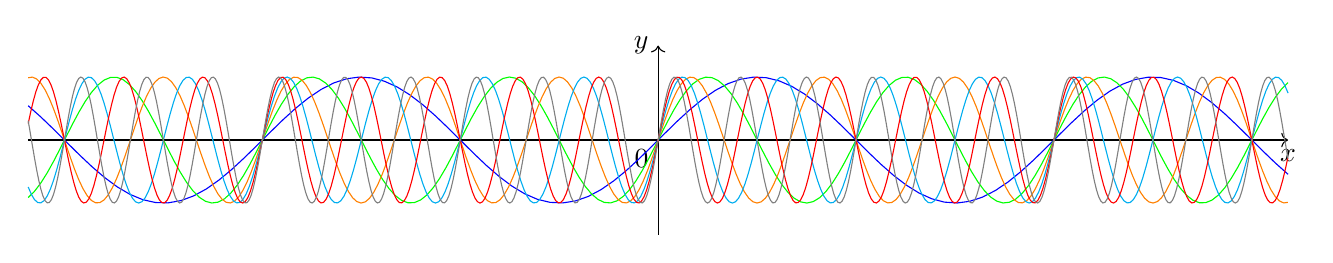
\begin{tikzpicture}[scale=.8]
\draw[->] (-10.,0)--(10.,0) node[below]{$x$};   
\draw[->] (0,-1.5)--(0,1.5)  node[left]{$y$};
\path
(0,0) node[below left]{$0$};
\draw[blue, domain=-10:10, samples=100, variable=\x] plot ({\x}, {(sin ( \x r))});
\draw[green, domain=-10:10, samples=200, variable=\x] plot ({\x}, {(sin ( 2 * \x r))});
\draw[orange, domain=-10:10, samples=300, variable=\x] plot ({\x}, {(sin ( 3 * \x r))});
\draw[cyan, domain=-10:10, samples=400, variable=\x] plot ({\x}, {(sin ( 4 * \x r))});
\draw[red, domain=-10:10, samples=500, variable=\x] plot ({\x}, {(sin ( 5 * \x r))});
\draw[gray, domain=-10:10, samples=600, variable=\x] plot ({\x}, {(sin ( 6 * \x r))});
\end{tikzpicture}
\end{center}
\caption{The sine function.}
\label{fig: 4.3}
\end{figure} \vspace{1 cm}
$$e^{-n \sqrt{x}} \leq 1 \qquad \forall n \in \mathbb{N} \qquad x \geq 1$$
\begin{figure}[!ht]
\begin{center}
\begin{tikzpicture}[scale=6.]
\draw[->] (-0.2,0)--(2.5,0) node[below]{$x$};   
\draw[->] (0,-0.2)--(0,0.5)  node[left]{$y$};
\path
(0,0) node[below left]{$0$};
\path
(0.5,0) node[below left]{$0.5$};
\path
(1.0,0) node[below left]{$1.0$};
\path
(1.5,0) node[below left]{$1.5$};ù
\path
(2.0,0) node[below left]{$2.0$};
\path
(2.5,0) node[below left]{$2.5$};
\foreach \i in {0,0.1, 0.2,...,2.5} \draw (\i,-0.02)--(\i,0.02);
\draw[blue, domain=1:2.5, samples=100, variable=\x] plot ({\x}, {(exp(- sqrt (\x)});
\draw[green, domain=1:2.5, samples=200, variable=\x] plot ({\x}, {(exp(-2 * sqrt (\x)});
\draw[orange, domain=1:2.5, samples=300, variable=\x] plot ({\x}, {(exp(-3 * sqrt (\x)});
\draw[red, domain=1:2.5, samples=400, variable=\x] plot ({\x}, {(exp(-4 * sqrt (\x)});
\end{tikzpicture}
\end{center}
\caption{The sequence of functions $e^{-n \sqrt{x}}$.}
\label{fig: 4.3}
\end{figure}
$$\star \leq |\frac{1}{x^3}| = \frac{1}{x^3} = g(x) \qquad \forall n \in \mathbb{N}$$
since $x \in [0, +\infty)$. Now we need to verify if $g \in L^1([0, +\infty))$. 
$$\int_1^{+\infty} |g(x)| dx = \int_1^{+\infty} |\frac{1}{x^3}| dx = \int_1^{+\infty} \frac{1}{x^3} dx < +\infty$$
since the summability criteria:
$$\int_1^{+\infty} \frac{1}{x^{\alpha}} dx = \begin{cases}
												\frac{1}{\alpha - 1} \qquad if \quad \alpha > 1 \\
												+\infty \qquad if \quad \alpha \leq 1
											\end{cases}$$
Now we can apply the Dominated Convergence Theorem (or Lebesgue Theorem):
$$\lim_{n \rightarrow +\infty} f_n(x) dx = \int_1^{+\infty} \lim_{n \rightarrow +\infty} f_n(x) dx = \int_1^{+\infty} \lim_{n \rightarrow +\infty} \frac{\sin(nx)}{x^3} e^{-n \sqrt{x}} dx = \int_1^{+\infty} 0 dx = 0.$$
Then the solution is
$$\lim_{n \rightarrow + \infty} \int_1^{+\infty} f_n(x) dx = \lim_{n \rightarrow +\infty} \frac{\sin(nx)}{x^3} e^{-n \sqrt{x}} dx = 0 \qquad \forall x \leq 1.$$
\clearpage
\chapter{$L^p$ Spaces}
\section*{Exercise $1$}
Analyze the convergence in $L^p([0, 1])$ with $1 \leq p < \infty$ of
$$f_n(x) = \frac{\cos(nx) e^{-n x}}{\sqrt[4]{x}} \qquad for \quad x \in [0, 1] \qquad \forall n \in \mathbb{N}.$$
For which $L^p$ the sequence converge to a certain function?
\section*{Solution}
\begin{figure}[!ht]
\begin{center}
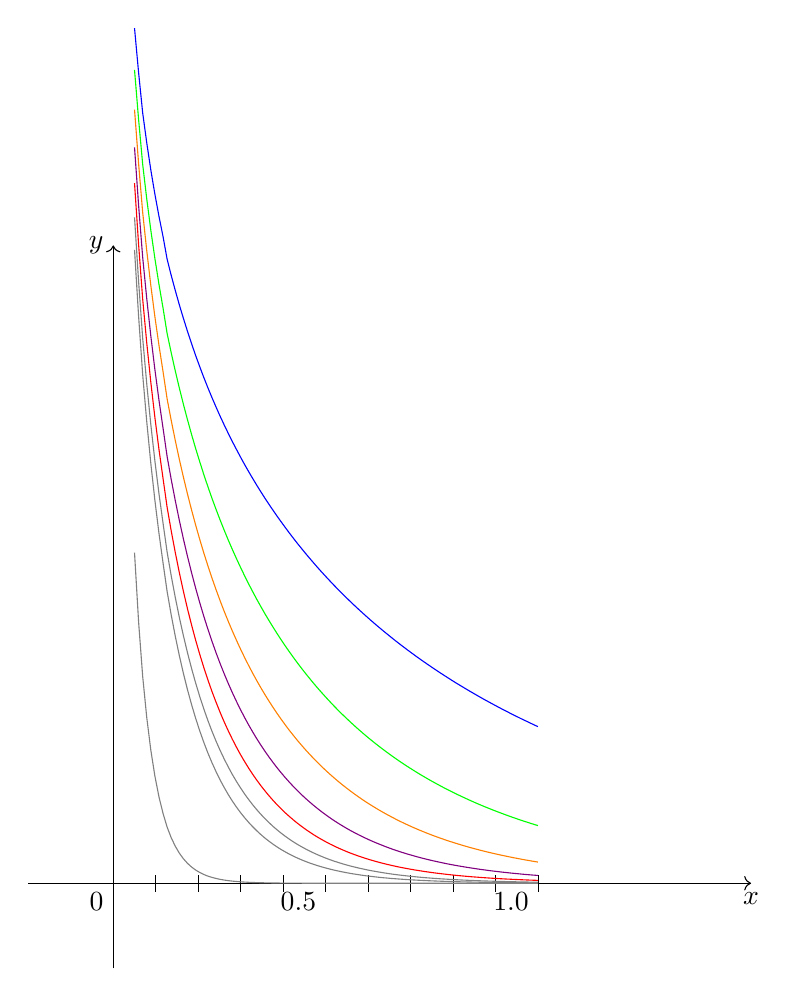
\begin{tikzpicture}[scale=5.4]
\draw[->] (-0.2,0)--(1.5,0) node[below]{$x$};   
\draw[->] (0,-0.2)--(0,1.5)  node[left]{$y$};
\path
(0,0) node[below left]{$0$};
\path
(0.5,0) node[below left]{$0.5$};
\path
(1.0,0) node[below left]{$1.0$};
\foreach \i in {0,0.1, 0.2,...,1.0} \draw (\i,-0.02)--(\i,0.02);
\draw[blue, domain=0.05:1.0, samples=100, variable=\x] plot ({\x}, {(cos (\x) / \x^(1 / 4) * exp(- \x)});
\draw[green, domain=0.05:1.0, samples=100, variable=\x] plot ({\x}, {(cos (2 * \x) / \x^(1 / 4) * exp(-2* \x)});
\draw[orange, domain=0.05:1.0, samples=100, variable=\x] plot ({\x}, {(cos (3 * \x) / \x^(1 / 4) * exp(- 3 * \x)});
\draw[violet, domain=0.05:1.0, samples=100, variable=\x] plot ({\x}, {(cos (4 * \x) / \x^(1 / 4) * exp(-4* \x)});
\draw[red, domain=0.05:1.0, samples=100, variable=\x] plot ({\x}, {(cos (5 * \x) / \x^(1 / 4) * exp(-5* \x)});
\draw[gray, domain=0.05:1.0, samples=100, variable=\x] plot ({\x}, {(cos (6 * \x) / \x^(1 / 4) * exp(-6* \x)});
\draw[gray, domain=0.05:1.0, samples=100, variable=\x] plot ({\x}, {(cos (7 * \x) / \x^(1 / 4) * exp(-7* \x)});
\draw[gray, domain=0.05:1.0, samples=100, variable=\x] plot ({\x}, {(cos (20 * \x) / \x^(1 / 4) * exp(-20* \x)});
\end{tikzpicture}
\end{center}
\caption{The sequence of functions $f_n(x)$.}
\label{fig: 4.3}
\end{figure}
First of all we search for which $p$ this sequence belongs to some $L^p$, applying the Dominated Convergence Theorem.
$$|f_n(x)| = |\frac{\cos(nx)}{\sqrt[4]{x}} e^{-n x}| \leq \frac{1}{\sqrt[4]{x}} = g(x) \qquad x \in [0, 1]$$
We know that $f_n(x)$ belongs to some $L^p$ if and only if
$$\int_0^1 |f_n(x)|^p dx < +\infty.$$
The exponents $p$ that satisfy this relations are the candidates.
$$\int_0^1 |f_n(x)|^p dx = \int_0^1 |\frac{\cos(nx)}{\sqrt[4]{x}} e^{-n x}|^p dx \leq \int_0^1 |\frac{1}{\sqrt[4]{x}}|^p dx = \int_0^1 \frac{1}{x^{\frac{p}{4}}} dx.$$
From the summability criteria:
$$\int_1^{+\infty} \frac{1}{x^{\alpha}} dx = \begin{cases}
												\frac{1}{\alpha - 1} \qquad if \quad \alpha > 1 \\
												+\infty \qquad if \quad \alpha \leq 1
											\end{cases},$$
since
$$|\frac{\cos(nx)}{\sqrt[4]{x}} e^{-n x}|^p \leq \bigl( \frac{1}{\sqrt[4]{x}} \bigl)^p$$
we have that for $p \in [1, 4) \qquad f_n(x) \in L^p([0, 1]) \qquad \forall n \in \mathbb{N}.$
\begin{itemize}
\item $f_n \in L^1([0, 1])$;
\item $f_n \in L^2([0, 1])$;
\item $f_n \in L^3([0, 1])$.
\end{itemize}
\textbf{Punctual Convergence}:
$$\lim_{n \rightarrow +\infty} f_n(x) = \lim_{n \rightarrow +\infty} \frac{\cos(nx)}{\sqrt[4]{x}} e^{-nx} = \lim_{n \rightarrow +\infty} \frac{\cos(nx)}{\sqrt[4]{x} e^{nx}} \rightarrow 0$$
so
$$f_n \rightarrow 0 \qquad \textrm{pointwise} \qquad \forall x \in [0,1],$$
we can apply the comparison criterium.
$$\lim_{x \rightarrow 0^+} f_n(x) \sqrt[4]{x} = \lim_{x \rightarrow 0^+} \frac{\cos(nx)}{\sqrt[4]{x}}e^{-nx} \sqrt[4]{x} = 1$$
$$f_n(x) \sim \frac{1}{\sqrt[4]{x}} \qquad \textrm{for} \qquad x \rightarrow 0^+.$$
Now we can analyze the convergence in $L^p([0, 1])$
$$\norm{f_n - f}_{L^p}$$
$$\norm{f_n(x) - f(x)}_{L^p([0, 1])}^p = \norm{f_n(x)}_{L^p([0,1])}^p = \norm{\frac{\cos(nx)}{\sqrt[4]{x} e^{nx}}}_{L^p([0,1])}^p = \int_0^1 |\frac{\cos(nx)}{\sqrt[4]{x} e^{-nx}}_{L^p([0,1])}|^p dx = \star$$
since
$$|\frac{\cos(nx)}{\sqrt[4]{x} e^{nx}}_{L^p([0,1])}|^p \leq g(x) = \frac{1}{x^{\frac{p}{4}}}$$
where
$$g \in L^p([0,1]) \qquad \textrm{for} \qquad 1 \leq p < 4,$$
we can apply the Dominated Convergence Theorem
$$\lim_{n \rightarrow +\infty} \norm{f_n(x) - f(x)}_{L^p([0, 1])}^p = \lim_{n \rightarrow +\infty} \int_0^1 |\frac{\cos(nx)}{\sqrt[4]{x}}e^{-nx}|^p dx = \int_0^1 \lim_{n \rightarrow +\infty} |\frac{\cos(nx)}{\sqrt[4]{x}} e^{-nx}|^p dx = 0.$$	
So
$$\lim_{n \rightarrow +infty} \norm{f_n(x) - f(x)}_{L^p([0, 1])} \rightarrow 0$$
$$f_n(x) \rightarrow 0 \qquad in \qquad L^p([0, 1]) \qquad \forall p \in [1; 4).$$
Since
$$\lim_{x \rightarrow 0^+} \frac{|f_n(x)|}{g(x)} = 1 \qquad \forall n \in \mathbb{N}$$
we have
$$f_n \in L^p([0, 1]) \leftrightarrow g \in L^p([0, 1])$$
so that
$$f_n \notin L^p([0, 1]) \qquad \textrm{if} \qquad p \geq 4.$$
The sequence $\{ f_n(x) \}_{n \in \mathbb{N}}$ can't converge in $L^p([0, 1])$ spaces if $p \geq 4$. \par 
In the case $p = +\infty$, we have
$$\norm{f_n(x)}_{\infty} = \esssup_{x \in (0, 1)} |\frac{\cos(nx)}{\sqrt[4]{x}}e^{-nx}| \leq \sup_{x \in (0,1)} |\frac{1}{\sqrt[4]{x}}| \rightarrow +\infty,$$
so
$$f_n \nrightarrow 0 \qquad \textrm{in} \qquad L^{\infty}((0, 1)).$$		
Since $[0, 1]$ is a bounded set we have the following embeddings:	
\begin{figure}[!ht]
\begin{center}
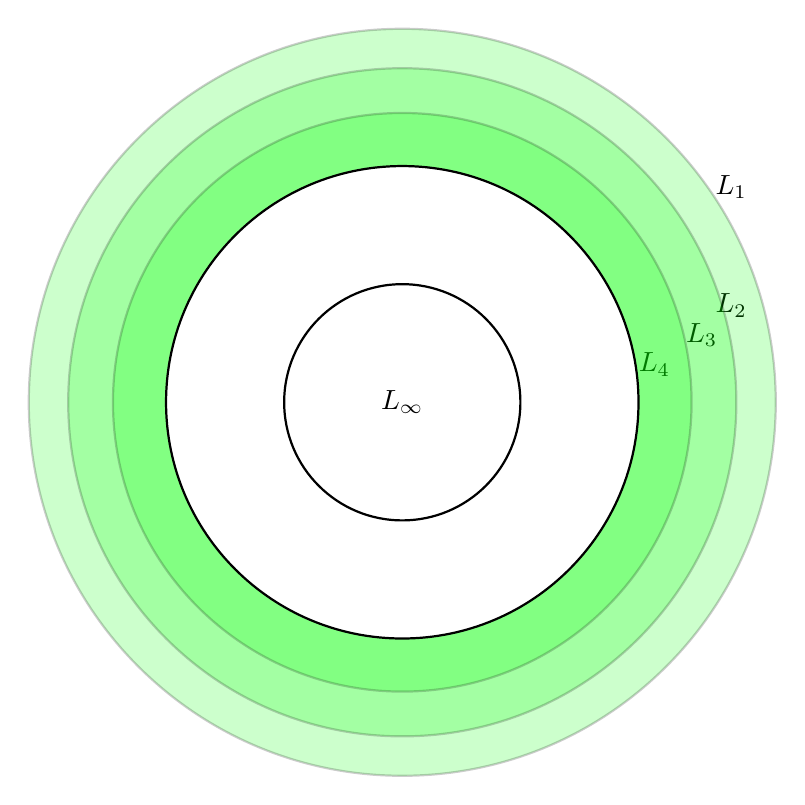
\begin{tikzpicture}[scale=1.5]
\path
(3,2) node[below left]{$\huge{L_1}$};
\path
(3.0,1) node[below left]{$\huge{L_2}$};
\path
(2.75,0.75) node[below left]{$\huge{L_3}$};
\path
(2.35,0.5) node[below left]{$\huge{L_4}$};
\path
(0.5,0.2) node[below left]{$\huge{L_{\infty}}$};
\draw[thick,black, fill=green, opacity=0.2] (0 ,0) circle({sqrt(10)});     
\draw[thick,black, fill=green, opacity=0.2] (0 ,0) circle({sqrt(8)});     
\draw[thick,black, fill=green, opacity=0.2] (0 ,0) circle({sqrt(6)});     
\draw[thick,black, fill=white, opacity=1.0] (0 ,0) circle({sqrt(4)});         
\draw[thick,black, fill=white, opacity=1.0] (0 ,0) circle({sqrt(1)}) node[text=black]{$\huge{L_{\infty}}$};;     
\end{tikzpicture}
\end{center}
\end{figure}							
The sequence $f_n(x)$ lives in "green" spaces.

\chapter{Hilbert Spaces}
\section*{Exercise $1$}
Let $X = (C(0,1); \norm{ \cdot }_{\infty})$ and consider
$$K = \{ f \in X : \int_0^{\frac{1}{2}} f(t) dt - \int_{\frac{1}{2}}^1 f(t) dt = 1 \}.$$
Show that $K$ is closed and not empty, and determine the projection of $0$ over the set $K$.
\section*{Solution}
$K$ is not empty. To show that we can take:
$$f(t) = \frac{\pi}{2} \sin(2 \pi t).$$
Now we can consider:
$$u(t) = \chi_{(0, \frac{1}{2})}(t) - \chi_{(\frac{1}{2}, 1}(t)$$
and consider the following operator:
$$(Tf) = \int_0^1 f u dt$$
where
$$T: C(0, 1) \rightarrow \mathbb{R}$$
$$K = T^{-1}(\{ 1 \})$$
since $\{ 1 \}$ is a singleton then it is closed; the contraimage of a closed set must be closed, so $K$ is closed.
$$|Tf| \leq C \norm{f}_{\infty}$$
$$f \in C(0, 1) \qquad \norm{f}_{\infty} \leq 1$$
then
$$f \notin K,$$
that is the elements of $K$ are of the form
$$\norm{ \cdot }_{\infty} > 1.$$
We have that 
$$f(x) \leq \norm{f}_{\infty} \leq 1 \qquad \forall x \in (0, 1)$$
"by contradiction"
$$f \in K \qquad \int_0^1 f u = 1$$
$$1 = \int_0^1 f u \leq \int_0^1 |f| |u| \leq \norm{f}_{\infty} \int_0^1 dt = \norm{f}_{\infty} \leq 1.$$
We have that
$$|f u| \leq 1 \qquad \int_0^1 |f u| = 1$$
so that
$$| f u | = 1 \quad a.e.$$
$$\int_0^1( 1 - | f u|) = 0 \qquad a.e.$$
so that
$$f u = 1 \qquad a.e. .$$
So we obtain this contradiction:
$$\begin{cases}
		f = 1 \qquad if \qquad x \in (0, \frac{1}{2}) \\
		f = -1 \qquad if \qquad x \in (\frac{1}{2}, 1)
  \end{cases}
$$
\begin{figure}[!ht]
\begin{center}
\begin{tikzpicture}[scale=2.0]
\draw[->] (-2.5,0)--(3.5,0) node[below]{$x$};   
\draw[->] (0,-1.5)--(0,1.5)  node[left]{$y$};
\draw[dashed] (0.5,-1.5)--(0.5,1.5);
\path
(0,0) node[below left]{$0$};
\path
(0.5,0) node[below left]{$0.5$};
\path
(1.0,0) node[below left]{$1.0$};
\foreach \i in {0,0.1, 0.2,...,1.0} \draw (\i,-0.02)--(\i,0.02);
\draw[blue, domain=-2.:0.5, samples=100, variable=\x] plot ({\x}, {1.});
\draw[blue, domain=0.5:3.0, samples=100, variable=\x] plot ({\x}, {-1.});
\end{tikzpicture}
\end{center}
\end{figure}
Now we consider:
$$d = \inf \{ \norm{ f }_{\infty} : f \in K \}$$
$$\norm{ f }_{\infty} \leq 1 \qquad \implies \qquad f \notin K$$
$$d = \inf \{ \norm{ f }_{\infty} : f \in K \} \geq 1,$$
we can take $1 < \alpha < 2$ and $\epsilon = \frac{\alpha - 1}{\alpha}$.
$$f_{\alpha} = -\frac{\alpha}{\epsilon}(x - \frac{1}{2})$$
\begin{figure}[!ht]
\begin{center}
\begin{tikzpicture}[scale=1.8]
\draw[->] (-2.5,0)--(3.5,0) node[below]{$x$};   
\draw[->] (0,-1.5)--(0,1.5)  node[above]{$y$};
\draw[dashed] (0.5,-1.5)--(0.5,1.5);
\path
(0,0) node[below left]{$0$};
\path
(0.5,0) node[below left]{$0.5$};
\path
(1.0,0) node[below left]{$1.0$};
\foreach \i in {0,0.1, 0.2,...,1.0} \draw (\i,-0.02)--(\i,0.02);
\draw[blue, domain=-2.:0.2, samples=100, variable=\x] plot ({\x}, {1.5});
\draw[blue, domain=0.2:0.8, samples=100, variable=\x] plot ({\x}, {-1.5 / 0.3 * (\x - 1. / 2.)});
\draw[green, domain=0.5:0.8, samples=100, variable=\x] plot ({\x}, {1.5 / 0.3 * (\x - 1. / 2.)});
\draw[blue, domain=0.8:2.0, samples=100, variable=\x] plot ({\x}, {-1.5});
\draw[green, domain=0.8:2.0, samples=100, variable=\x] plot ({\x}, {1.5});
\end{tikzpicture}
\end{center}
\end{figure}
\clearpage
Now we show that $f_{\alpha} = -\frac{\alpha}{\epsilon}(x - \frac{1}{2})$ belongs to $K$.
$$\int_0^{\frac{1}{2}} f_{\alpha} - \int_{\frac{1}{2}}^1 f_{\alpha} = 1 \qquad \forall \alpha \in (1, 2)$$
$$\norm{f_{\alpha}}_{\infty} = \alpha,$$
$\alpha$ is the supremum,
$$d = \inf \{ \norm{f}_{\infty} : f \in K \} \leq \norm{f_{\alpha}}_{\infty} = \alpha$$
$$\alpha \in (1, 2)$$
$$\begin{cases}
	d \leq 2 \\
	\forall \alpha \in (1,2)
  \end{cases} \implies d \leq 1$$
so that
$$d = \inf \{ \norm{ f }_{\infty} : f \in K \} = 1,$$
but this $\inf$ is not assumed, this is not a minimum, then
$$\nexists f \in K \qquad \textrm{s.t.} \qquad d = \norm{f}_{\infty} = 1,$$
$$d = d(0, K)$$
$$0 \notin K.$$
\clearpage
\chapter{Operators}
\section*{Exercise $1$}
Let 
$$a(x) = \begin{cases}
			x \qquad if \quad x \in (0, \frac{1}{2}] \\
			0 \qquad if \quad x \in (\frac{1}{2}, 1]
		 \end{cases}$$
and consider the operator
$$T : L^2(0, 1) \rightarrow L^2(0, 1)$$
given by
$$Tf(x) = a(x) f(x), \qquad x \in (0, 1).$$
Show that $T \in \mathcal{L}(L^2[0,1])$ and compute $\norm{T}$.
\section*{Solution}
\begin{figure}[!ht]
\begin{center}
\begin{tikzpicture}[scale=2.0]
\draw[->] (-2.5,0)--(3.5,0) node[below]{$x$};   
\draw[->] (0,-1.5)--(0,1.5)  node[left]{$y$};
\draw[dashed] (0.5,-1.5)--(0.5,1.5);
\path
(0,0) node[below left]{$0$};
\path
(0.5,0) node[below left]{$0.5$};
\path
(1.0,0) node[below left]{$1.0$};
\path
(1.0,1.0) node[below left]{$a(x)$};
\foreach \i in {0,0.1, 0.2,...,1.0} \draw (\i,-0.02)--(\i,0.02);
\draw[red, domain=0.:0.5, samples=100, variable=\x] plot ({\x}, {\x});
\draw[red, domain=0.5:1.0, samples=100, variable=\x] plot ({\x}, {0.});
\end{tikzpicture}
\end{center}
\end{figure}
$$f \in L^2(0, 1)$$
$$\norm{T f}_{L^2(0, 1)}^2 = \int_0^1 a(x)^2 f(x)^2 dx \leq \frac{1}{4} \int_0^1 f(x)^2 dx = \frac{1}{4} \norm{f}_{L^2(0,1)}^2$$
so that
$$\norm{T}_{\mathcal{L}(L^2(0,1))} \leq \frac{1}{2}.$$
Then we want to show that $\frac{1}{2}$ is the value of the norm, that is
$$\norm{T} = \frac{1}{2}.$$
We define
$$f_n(x) = \begin{cases}
			\sqrt{n} \qquad if \quad x \in [\frac{1}{2} - \frac{1}{n}, \frac{1}{2}], \qquad n \geq 2 \\
			0 \qquad \textrm{otherwise}
		   \end{cases}$$
\begin{figure}[!ht]
\begin{center}
\begin{tikzpicture}[scale=2.0]
\draw[->] (-2.5,0)--(3.5,0) node[below]{$x$};   
\draw[->] (0,-1.5)--(0,3.5)  node[left]{$y$};
\draw[dashed] (0.5,-1.5)--(0.5,3.5);
\path
(0,0) node[below left]{$0$};
\path
(0.5,0) node[below left]{$0.5$};
\path
(1.0,0) node[below left]{$1.0$};
\path
(1.0,1.0) node[below left]{$f_n(x)$};
\foreach \i in {0,0.1, 0.2,...,1.0} \draw (\i,-0.02)--(\i,0.02);
\draw[red, domain=0.:0.5, samples=100, variable=\x] plot ({\x}, {sqrt (2)});
\draw[red, domain=1./6:0.5, samples=100, variable=\x] plot ({\x}, {sqrt (3)});
\draw[red, domain=1./4:0.5, samples=100, variable=\x] plot ({\x}, {sqrt (4)});
\draw[red, domain=3./10:0.5, samples=100, variable=\x] plot ({\x}, {sqrt (5)});
\draw[red, domain=1./3:0.5, samples=100, variable=\x] plot ({\x}, {sqrt (6)});
\draw[red, domain=5./14:0.5, samples=100, variable=\x] plot ({\x}, {sqrt (7)});
\draw[red, domain=0.5:1.0, samples=100, variable=\x] plot ({\x}, {0.});
\draw[->] (0.1,-0.5)--(0.45,-0.5);
\path
(0.1, -0.6) node[below]{$\frac{1}{2} - \frac{1}{n}$};
\end{tikzpicture}
\end{center}
\end{figure}
$$\norm{f_n(x)}_{L^2(0,1)}^2 = \int_0^1 f_n(x)^2 = 1$$
Now we compute the norm of the image:
$$\norm{T f_n(x)}_{L^2(0,1)}^2 = \int_0^1 a(x)^2 f_n(x)^2 dx \geq \star$$
we can minor the integral with
$$\star \geq \int_{\frac{1}{2} - \frac{1}{n}}^{\frac{1}{2}} n(\frac{1}{2} - \frac{1}{n})^2 dx = (\frac{1}{2} - \frac{1}{n})^2 \rightarrow \frac{1}{4} \qquad \textrm{for} \quad n \rightarrow +\infty$$
so that
$$\norm{T}_{\mathcal{L}(L^2(0,1))} = \frac{1}{2}.$$
We can characterize the norm in various ways.
$$\norm{T}_{\mathcal{L}(L^2(0,1))} = \sup_{f \in L^2(0,1) \quad \norm{f}_{L^2} = 1} \frac{\norm{Tf}_{L^2(0,1)}}{\norm{f}_{L^2(0,1)}} \leq \frac{1}{2}.$$
We have shown that 
$$\norm{Tf_n(x)}_{L^2(0,1)}^2 \geq \frac{1}{4},$$
that is
$$\norm{T f_n(x)}_{L_2(0,1)} \geq \frac{1}{2},$$
but at the same time we have
$$\norm{T} \leq \frac{1}{2}$$
then
$$\norm{T f_n(x)} = \frac{1}{2}.$$
\clearpage
\section*{Exercise $2$}
Let $(f'_h)_{h \in \mathbb{N}} \in L^p$ for some $p$, with the following hypotheses:
\begin{itemize}
\item $(f'_h)_{h \in \mathbb{N}}$ is bounded in $L^p$ for some $p$;
\item $f_h(0)$ is bounded.
\end{itemize}
Show that $(f_h)_{h \in \mathbb{N}}$ is compact (relatively) in $(C([0,1]), \norm{\cdot}_{\infty}$.
\section*{Solution}
From the hypotheses we can suppose that
$$f_h(x) = f_h(0) + \int_0^x f'_h(y) dy \qquad x \in [0, 1].$$
Since we have to show the compactness in the set of continuous fuunctions we need to utilize the Ascoli-Arzel\`{a} theorem. \par
Let $C > 0$ constant. \par 
\textbf{Equiboundedness}
$$h \in \mathbb{N}, \qquad x \in [0, 1]$$
$$|f_h(x)| \leq |f_h(0)| + \int_0^x |f'_h(y)| dy \leq \star$$
using the hypothesis $2$ and the H\"{o}lder inequality
$$\star \leq C + \norm{f'_h}_{L^p(0,1)} x^{\frac{1}{p'}} \leq M$$
so that
$$|f_h(x)| \leq M,$$
that is $f_h$ is equibounded. \par   
\textbf{Equicontinuity}
$$x, y \in [0, 1], \qquad x < y$$
$$f_h(y) - f_h(x) \leq \int_x^y |f'_h(w)| dw \leq \star$$
using the H\"{o}lder inequality
$$\star \leq \norm{f'_h}_{L^p(0,1)}|y - x|^{\frac{1}{p'}}.$$
This shows that the fuunctions $f_h$ are equi-h\"{o}lder  with exponent $\frac{1}{p'}$, in particular they are eqicontinuous. \par   
Then from the Ascoli-Arzel\`{a} theorem they are relatively compact.

\end{document}